\documentclass[a4j,uplatex,titlepage]{jsarticle}
\usepackage{amsmath,amssymb}
\usepackage[dvipdfm]{graphicx}
\usepackage[hyphens]{url}
\usepackage[dvipdfmx]{xcolor}
\usepackage{listings,jvlisting} 
\usepackage{comment}
\urlstyle{same}
\setlength{\parindent}{0pt}

\renewcommand{\figurename}{Fig.}

\begin{document}
\title{レポート}
\author{\texttt{名前名前}}
\date{\today}
\maketitle
\clearpage

\tableofcontents
\clearpage


\section{概要}
こんにちわ!
\subsection{数式}
数式\cite{eq1}を書いてみよう!
\begin{multline}
    a+b+c+d+e+f \\
    -g-h-i+j+k-l-m+n \\
    -o-p-q-r-s+t+u \\
    +v+w+x-y-z
\end{multline}

\begin{eqnarray}
    (x - 3)(x + 2)(x + 7) &=& (x - 3)(x^2 + 9x + 14) \\
    &=& (x^3 + 9x^2 + 14x) - (3x^2 + 27x + 42) \\
    &=& x^3 + 6x^2 - 13x - 42
\end{eqnarray}

以下は式番号を記述しない場合。
\begin{eqnarray*}
    (x - 3)(x + 2)(x + 7) &=& (x - 3)(x^2 + 9x + 14) \\
    &=& (x^3 + 9x^2 + 14x) - (3x^2 + 27x + 42) \\
    &=& x^3 + 6x^2 - 13x - 42 
\end{eqnarray*}

以下は部分的に式番号を記述する場合。
\begin{eqnarray}
    (x - 3)(x + 2)(x + 7) &=& (x - 3)(x^2 + 9x + 14) \nonumber\\
    &=& (x^3 + 9x^2 + 14x) - (3x^2 + 27x + 42) \nonumber\\
    &=& x^3 + 6x^2 - 13x - 42 
\end{eqnarray}

\begin{eqnarray}
    \frac{\partial E}{\partial w^{k,k+1}_{1,1}}\nonumber\\
    &=& \frac{\partial E}{\partial i^{k+1}_1} \frac{\partial i^{k+1}_1}{\partial w^{k,k+1}_{1,1}}\nonumber\\
    &=& \frac{\partial E}{\partial o^{k+1}_1} \frac{\partial o^{k+1}_1}{\partial i^{k+1}_1} \frac{\partial i^{k+1}_1}{\partial w^{k,k+1}_{1,1}}\nonumber\\
    &=& (o^{k+1}_1 - t)f'(i^{k+1}_1)o^{k}_1
\end{eqnarray}

\section{画像}
画像を貼るよ。位置指定方法は\ref{画像の位置指定方法}に示す。
\begin{table}[h]
    \begin{center}
      \caption{{画像の位置指定方法}\label{画像の位置指定方法}}
      \scalebox{0.7}[0.9]{
        \begin{tabular}{|c|r|} \hline
          h & 記述した部分 \\ \hline
          t & ページの上部 \\ \hline
          b & ページの下部 \\ \hline
          p & 独立したページ \\ \hline
        \end{tabular}
      }
    \end{center}
  \end{table}

\subsection{png}
\cite{png}←参考にした。\ref{fig:one}がpngの画像。
\begin{figure}[h]
    \begin{center}
    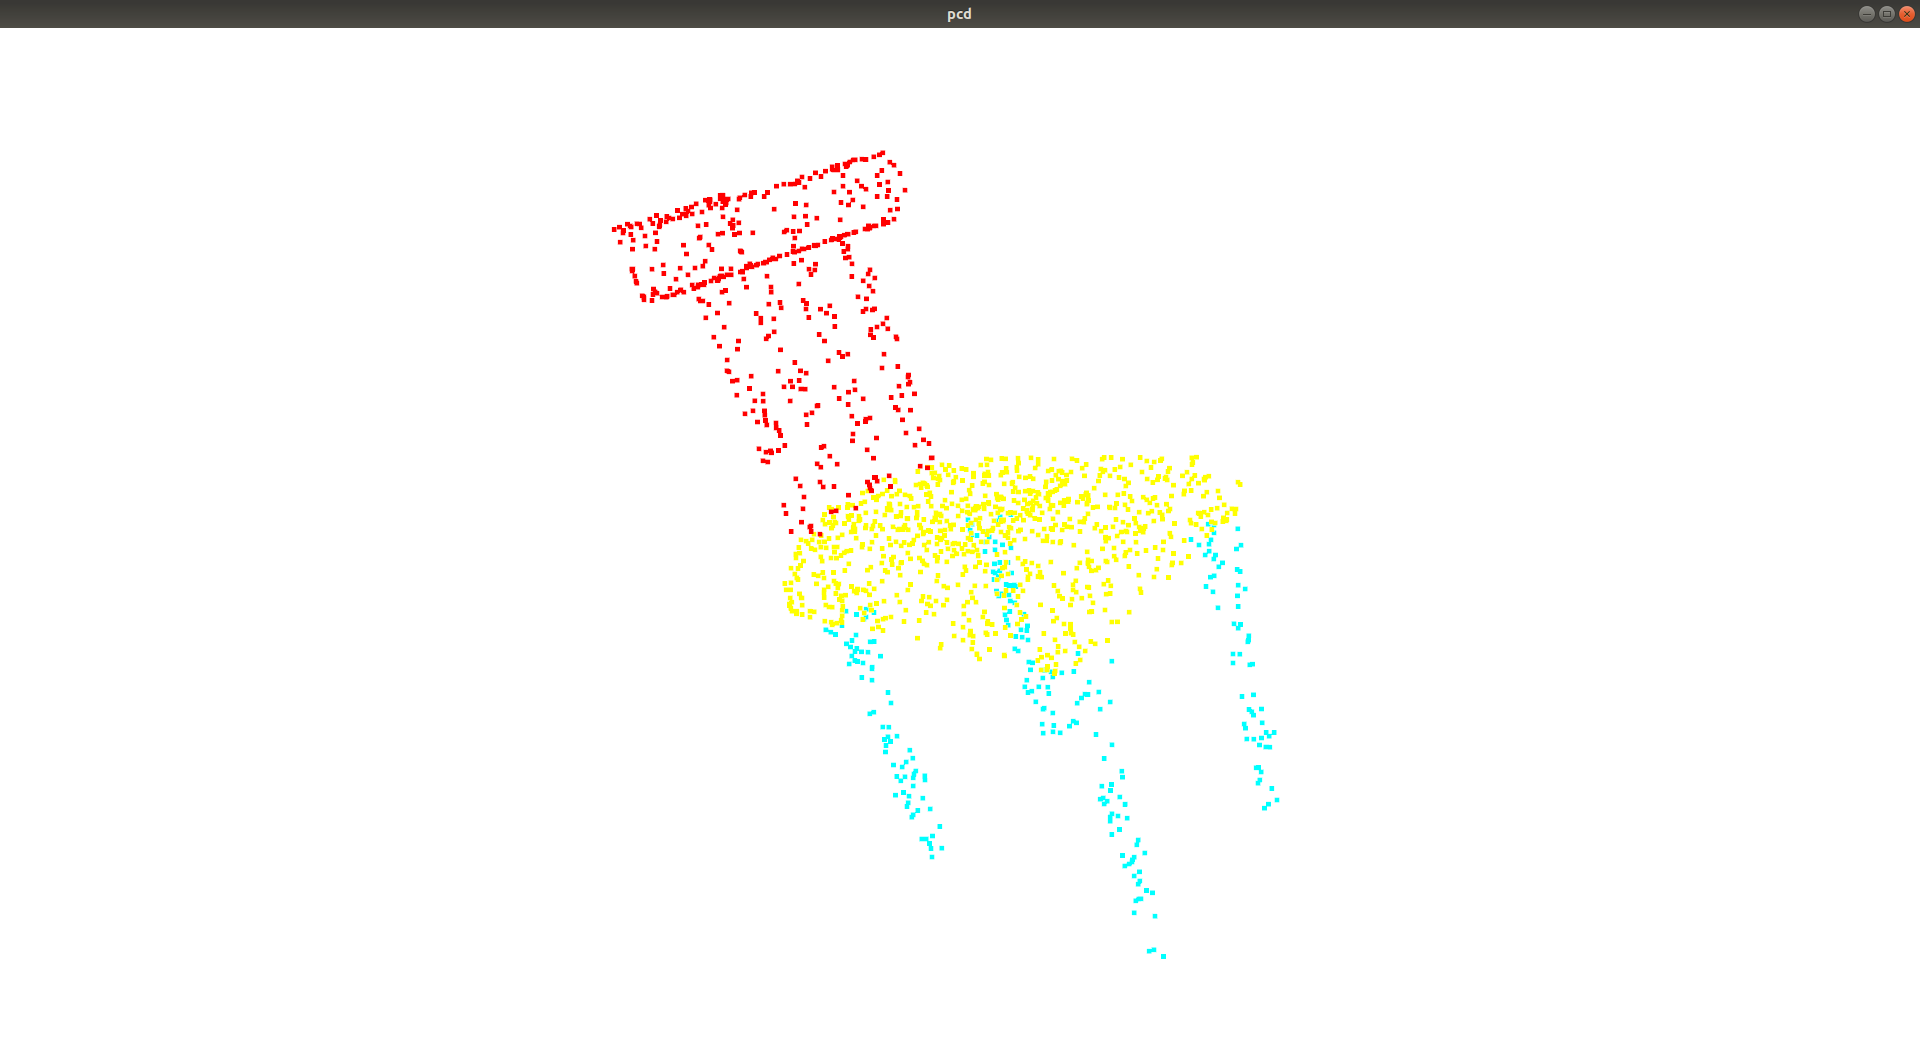
\includegraphics[width=8cm]{figure/pcl.png}
    \end{center}
    \caption{hにすることで記述した位置に図が配置される}
    \label{f1}
\end{figure}

\begin{figure}[tb]
    \begin{center}
    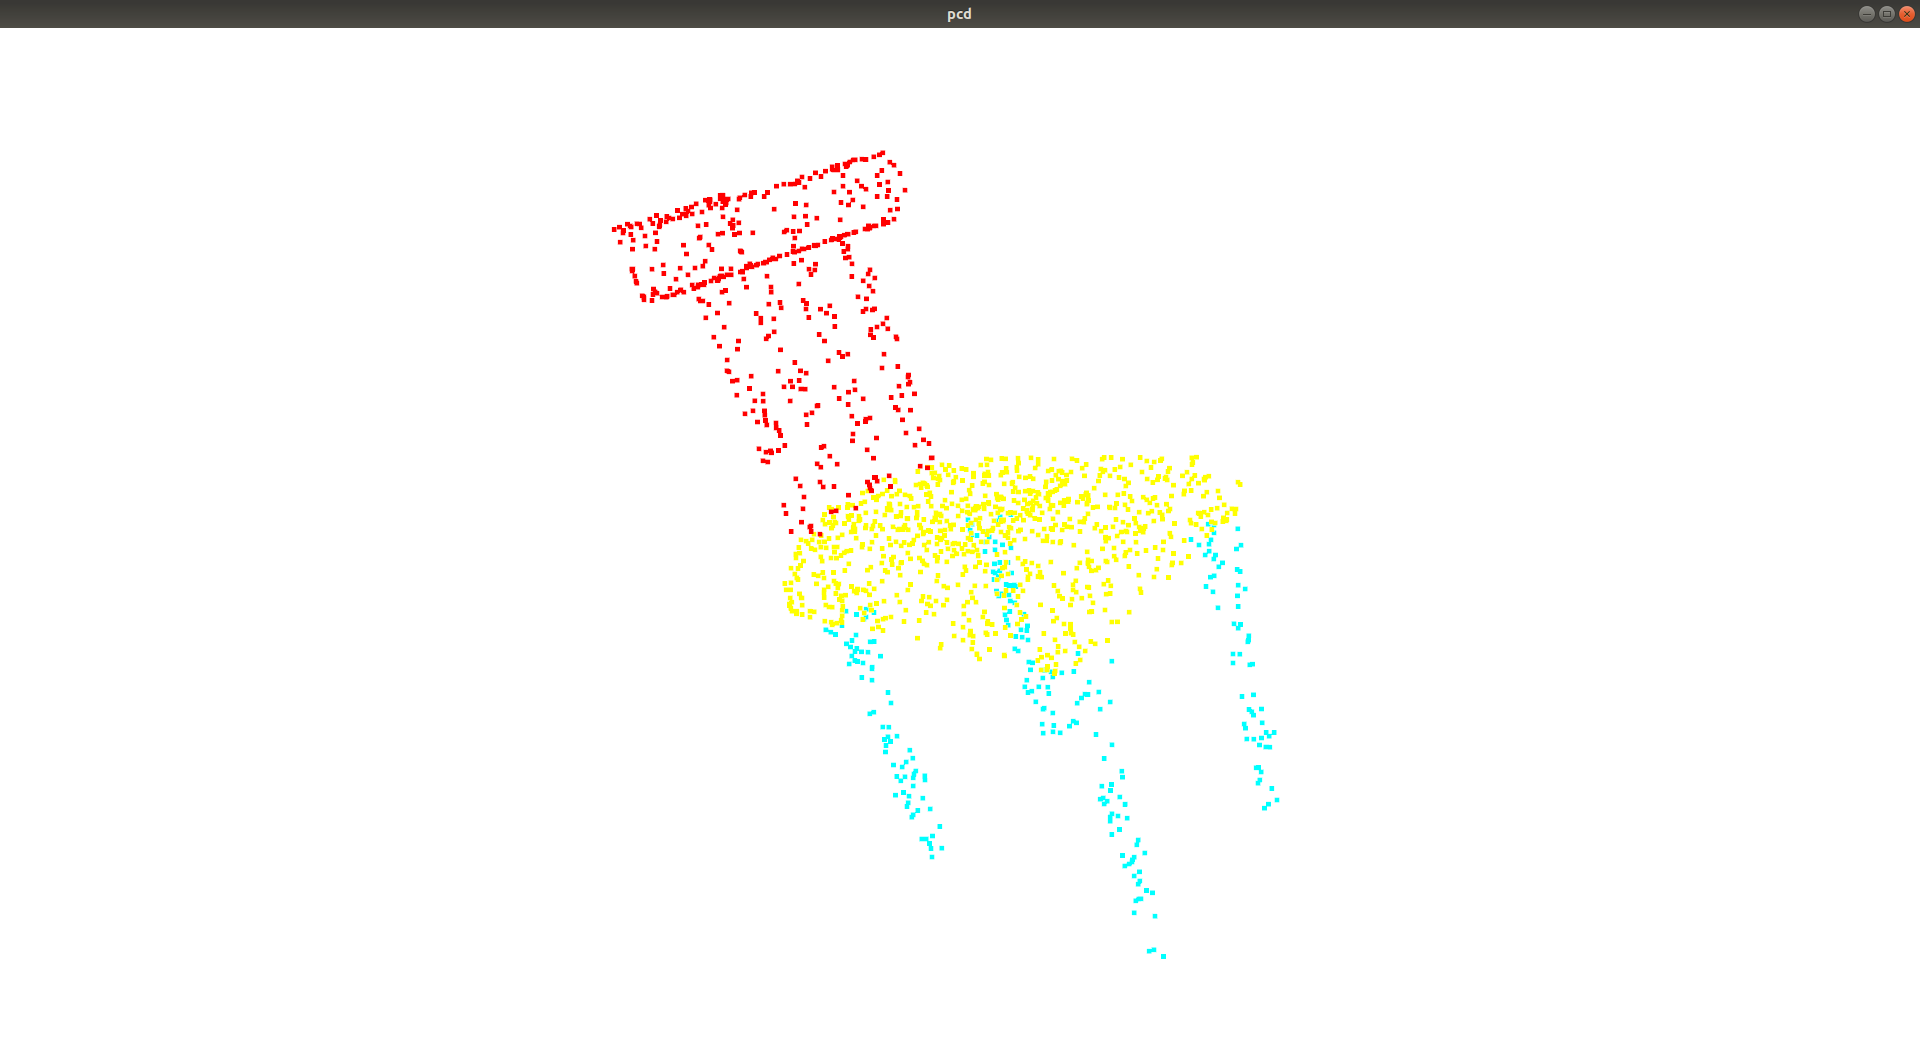
\includegraphics[width=8cm]{figure/pcl.png}
    \end{center}
    \caption{tbをつけることで図の位置がtopかbottomのどちらかになる}
    \label{fig:one}
\end{figure}

\begin{figure}[tb]
    \begin{minipage}[b]{0.48\columnwidth}
      \centering
      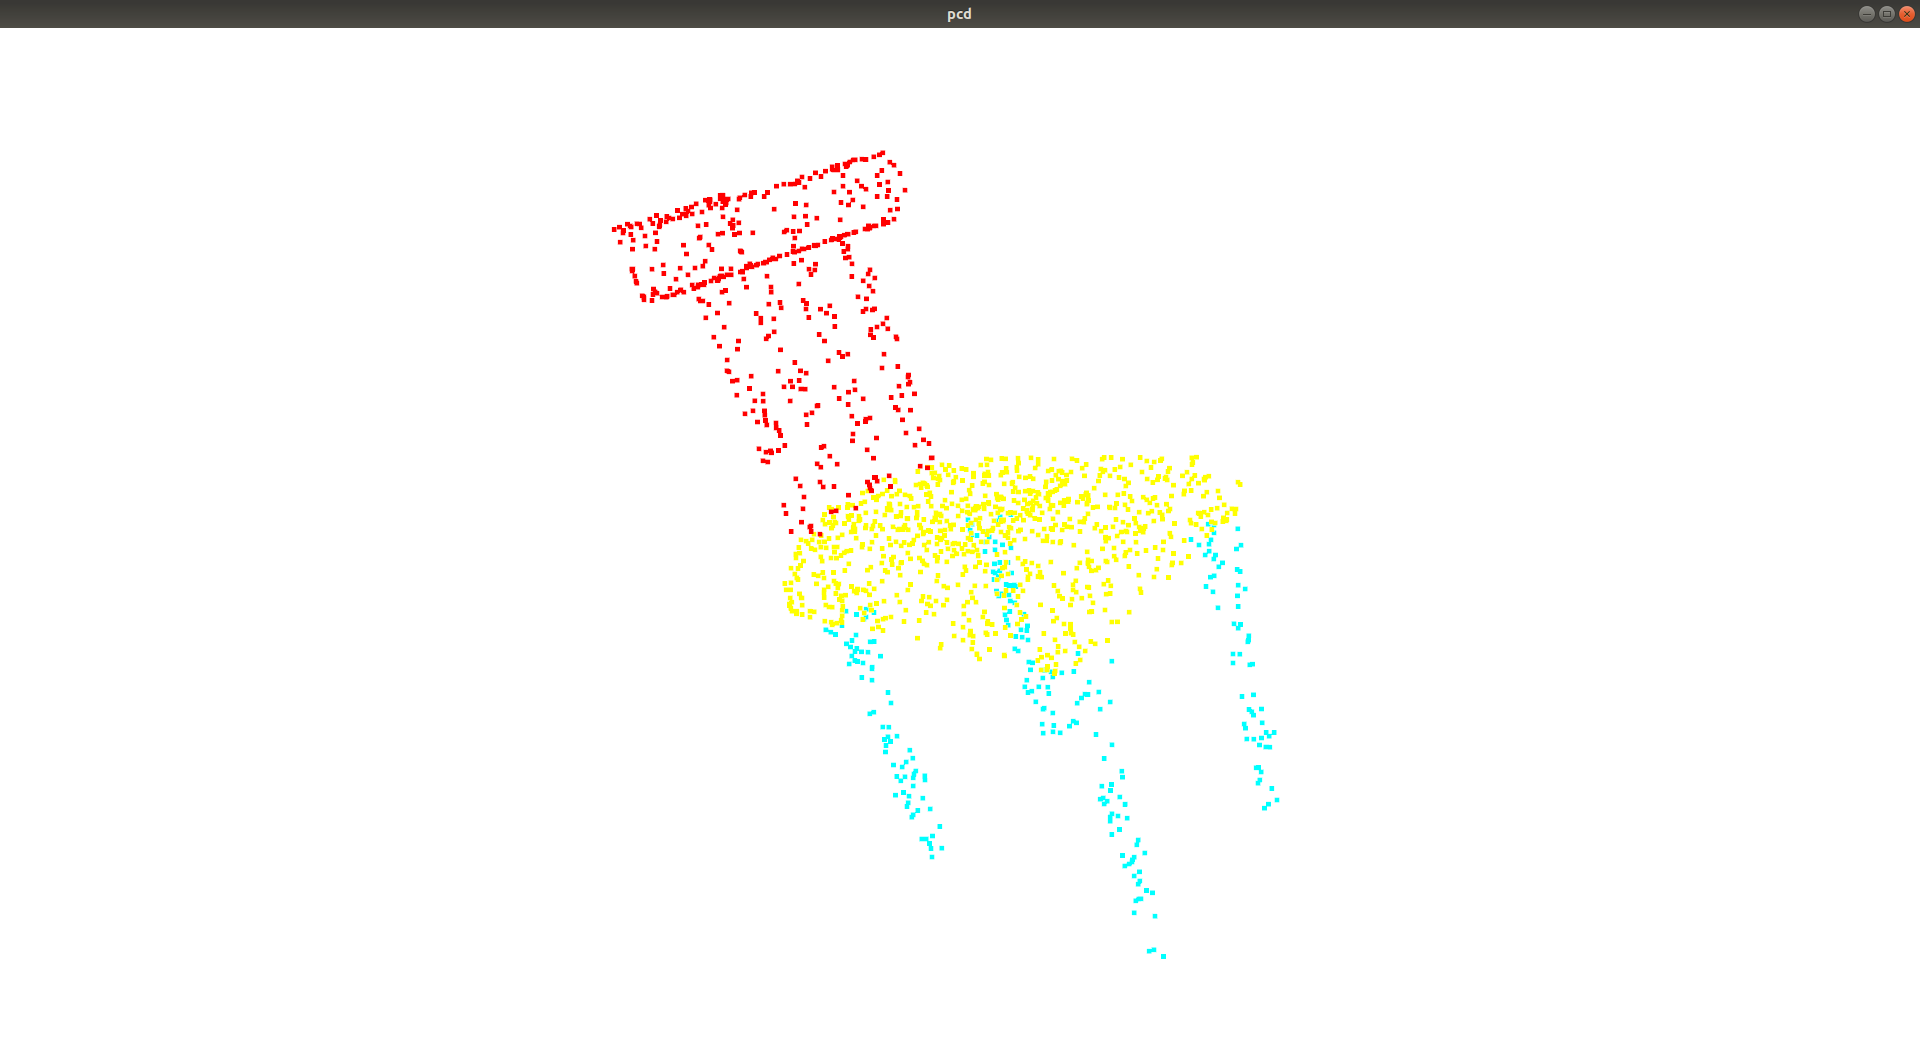
\includegraphics[width=8cm]{figure/pcl.png}
      \caption{画像①です}
    \end{minipage}
    \hspace{0.04\columnwidth} % ここで隙間作成
    \begin{minipage}[b]{0.48\columnwidth}
      \centering
      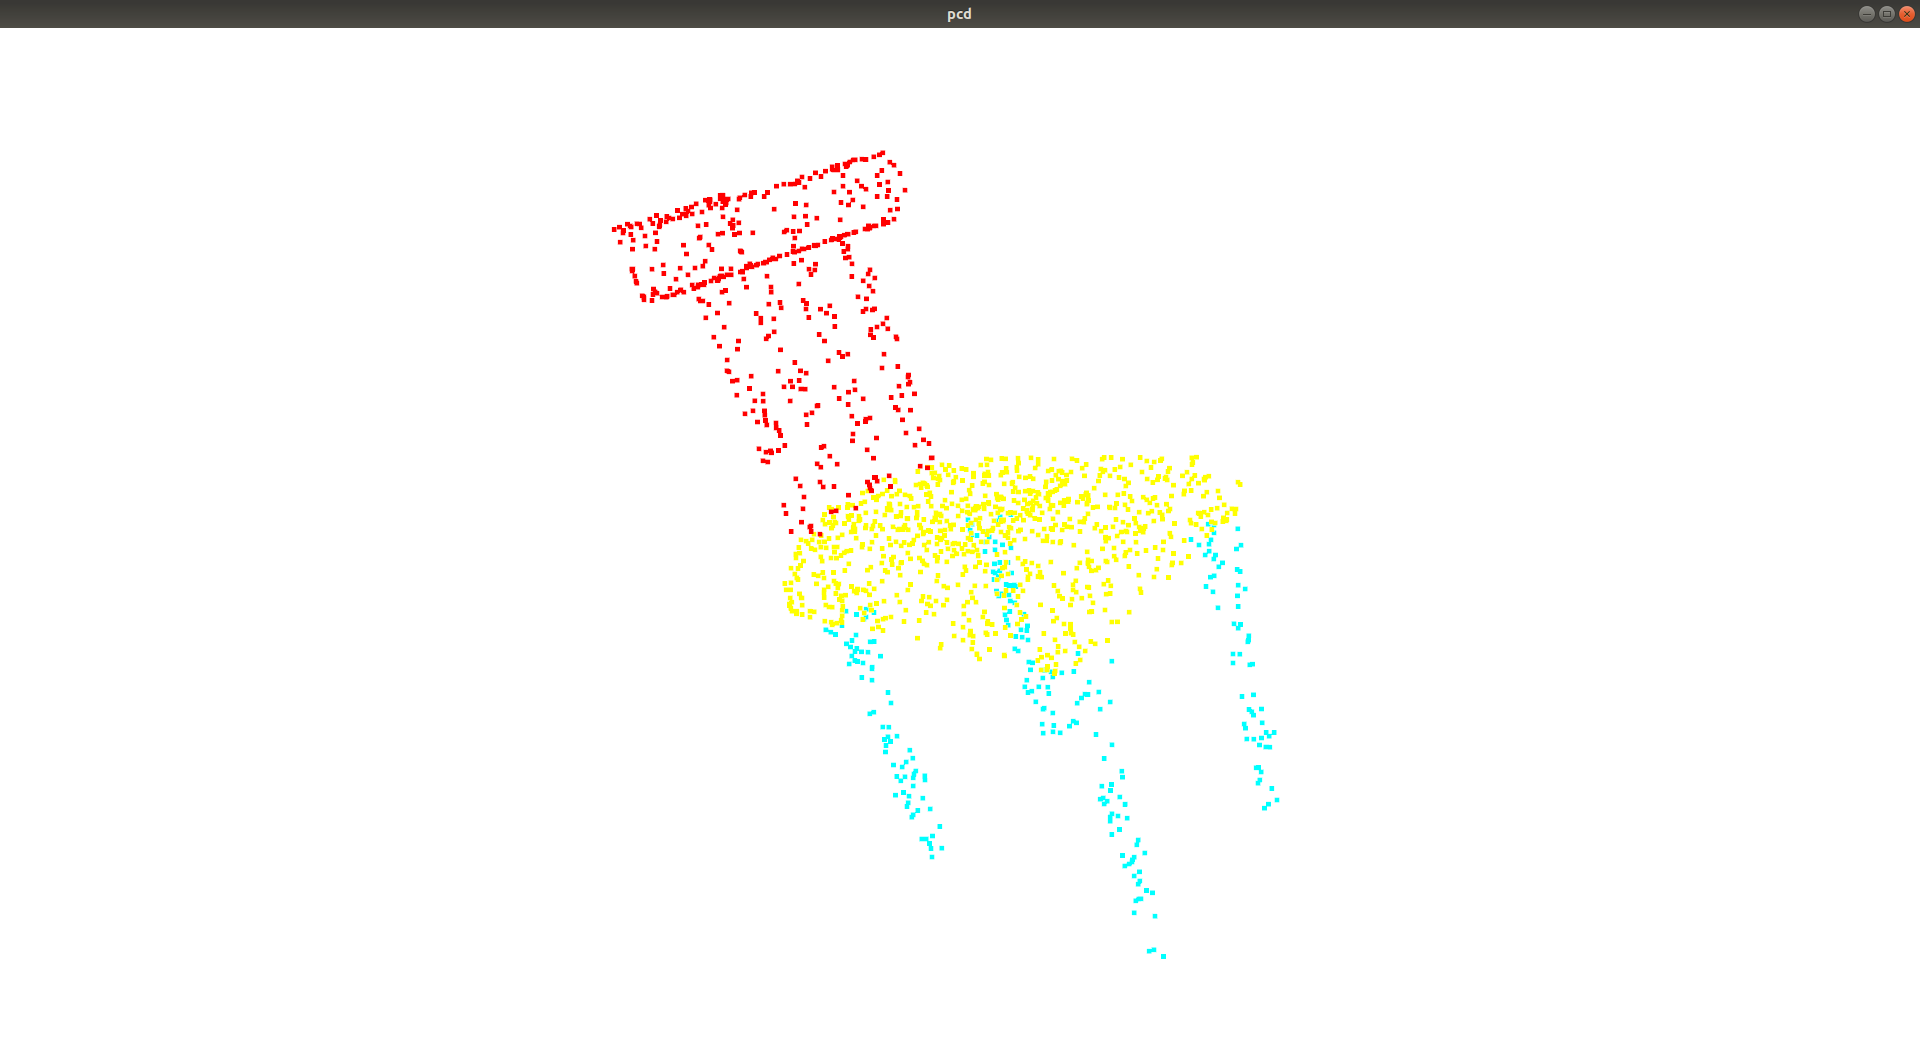
\includegraphics[width=8cm]{figure/pcl.png}
      \caption{画像②です}
    \end{minipage}
  \end{figure}

\section{その他}
\subsection{箇条書き}
\begin{itemize}
    \item (A) Feature-based approach\\ 
    \item (B) Marker-based approach\mbox{}\\
    ほげほげほげ
    \item (C) Simulation-based approach\\ 
    \item (D) Special devices and environmental approaches:\mbox{}\\
    ふがふがふが 
\end{itemize}

\subsection{色を変える}
\color{red}赤色赤色赤色赤色赤色\color{black}\\
\color{blue}赤色赤色赤色赤色赤色\color{black}
\subsection{ソースコード}
\lstset{
  basicstyle={\ttfamily},
  identifierstyle={\small},
  commentstyle={\smallitshape},
  keywordstyle={\small\bfseries},
  ndkeywordstyle={\small},
  stringstyle={\small\ttfamily},
  frame={tb},
  breaklines=true,
  columns=[l]{fullflexible},
  numbers=left,
  xrightmargin=0zw,
  xleftmargin=3zw,
  numberstyle={\scriptsize},
  stepnumber=1,
  numbersep=1zw,
  lineskip=-0.5ex
}
HelloWorldのソースコードを,ソースコード\ref{src1}に示す.
\begin{lstlisting}[caption=C,label=src1]
#include<stdio.h>
int main(){
   printf("Hello world!");
}
\end{lstlisting}

\begin{lstlisting}[caption=Python,label=src1]
for num in range(20):
print num
if num == 10
    break
\end{lstlisting}

\clearpage

\begin{thebibliography}{99}
\bibitem{eq1} 数式1、https://uec.medit.link/latex/eqnalign.html
\bibitem{png} 画像1、\url{https://qiita.com/kaizen_nagoya/items/3d188cbeeaa844f880b0}
\bibitem{url} URL1、\url{https://ja.tak-cslab.org/archives/901}
\end{thebibliography}
\end{document}